%----------------------------------------------------------------------------------------
%	SOLUTION 3.a
%----------------------------------------------------------------------------------------
\subsection*{Solution 3.a}
\paragraph{Summary:} Here Tensorflow is used to build a convolutional neural network as asked in the homework. The network is learned using stochastic gradient descent (SGD) as the optimizer to update the weights without momentum and with a learning rate of $0.01$. The parameters are tuned after iterating through multiple runs with different learning rates. The value which produced best accuracy is used. I have used batch normalization layer after convolution layer to normalize the output of the convolution layer. Batch normalization is actually standardization procedure over mini batches where the convolved ensemble feature mean is subtracted from each feature and divided by the standard deviation of corresponding feature. It helps in improving the accuracy. Once the output is normalized, I have used the ReLU activation layer. Another alternative to this could be to directly pass the \textit{activation='relu'} argument to convolution layer in Tensorflow Keras.

For SGD, I have used learning rate of $0.01$ with no momentum. For ADAGRAD, I have used learning rate of $0.1$ with initial accumulator value of $0.01$. For ADAM, I have used learning rate of $0.001$ and $\rho_1$ and $\rho_2$ values of $0.9$ and $0.999$ respectively. I ran the code multiple times with different set of hyperparameters and the chose the values which produced best accuracy. For ADAM, it seemed to me that the default values gave me the best result. I have also converted labels to \textit{one-hot} representation to use \textit{categorical crossentropy} as the loss for Tensorflow model. The input features are scaled to $[0, 1]$ as I have seen this improves the performance of the neural network a lot.
\paragraph{Convergence criteria used:} I have declared convergence if in $3$ consecutive epochs the decrease of loss is less than $0.001$ or loss increases for $3$ consecutive epochs. The maximum number of epochs has a limit of $100$ though I have never seen hitting this limit before convergence is achieved.
%----------------------------------------------------------------------------------------
%	SOLUTION 3.a
%----------------------------------------------------------------------------------------
\paragraph{Results:} Fig.~\ref{fig:q3_sgd_loss_acc} shows the cumulative loss and accuracy with increasing nuber of epochs.
%%%%%%%%%%%%%%%%%%%%%%% SGD LOSS + ACCURACY %%%%%%%%%%%%%%%%%%%%%
\begin{figure}[!h]
	\centering
	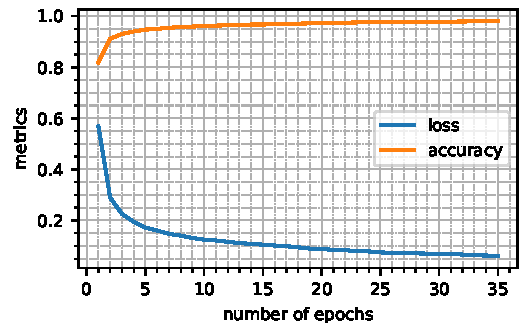
\includegraphics[scale=1.0,trim={0cm 0cm 0cm 0cm},clip]{./code/generatedPlots/q3_sgd_loss_acc.pdf}
	\caption{Q3: SGD cumulative training loss and accuracy with different epochs: CNN}
	\label{fig:q3_sgd_loss_acc}
\end{figure}
From Fig.~\ref{fig:q3_sgd_loss_acc}, we can see that as we increase the number of epochs, the network learns better and thus the loss decreases monotonically and the accuracy increases. Table~\ref{tbl:q3_sgd_loss_acc} shows the training loss and accuracy after convergence and test loss and accuracy.
%%%%%%%%%%%%%%%%%%%%%%%%%% TRAIN+TEST %%%%%%%%%%%%%%%%%%%%%%%%%%%%%%%%%%%
\begin{table}[ht]
	\centering
	\caption{Q3: Train (after convergence) and test loss and accuracy}
	\begin{tabular}[t]{ccc} 
		\hline
		& Loss & Accuracy(\%)\\ [0.5ex] 
		\hline
		Train 	& $0.060$ 	& $98.04$\\
		Test 	& $0.032$ 	& $98.93$\\[1ex]
		\hline
	\end{tabular}
	\label{tbl:q3_sgd_loss_acc}
\end{table}
If we compare the results shown in Table~\ref{tbl:q2_sgd_loss_acc} with that of Table~\ref{tbl:q3_sgd_loss_acc}, we can see that though feed forward network gave a slightly better accuracy for training data, CNN gave better test accuracy.
%----------------------------------------------------------------------------------------
%	SOLUTION 3.b
%----------------------------------------------------------------------------------------
\subsection*{Solution 3.b}
\paragraph{Convergence time calculation:} I have calculated the convergence time in seconds using the Tensorflow callbacks which is essentially the time between the train end and train begin callbacks. I have measured the time using \textit{time.time()} module of Python. Also, I have averaged the time over $10$ independent runs to reduce the variability.
\paragraph{Results:} Fig.~\ref{fig:q3_sgd_conv_time}, Fig.~\ref{fig:q3_adagrad_conv_time} and Fig.~\ref{fig:q3_adam_conv_time} show the evolution of convergence time, averaged over $10$ runs, with increasing batch size. 
%%%%%%%%%%%%%%%%%%%%%%% CONVERGENCE TIME %%%%%%%%%%%%%%%%%%%%%
\begin{figure}[!h]
	\centering
	\subfloat[][SGD: Convergence time, averaged over 10 runs, with increasing batch size]{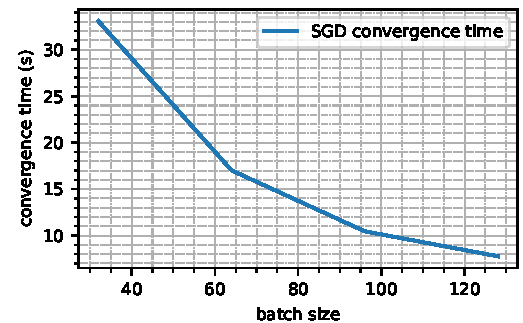
\includegraphics[scale=0.97,trim={0cm 0cm 0cm 0cm},clip]{./code/colabPlots/q3_sgd_conv_time.pdf}\label{fig:q3_sgd_conv_time}}\hspace{0.5cm}
	\subfloat[][ADAGRAD: Convergence time, averaged over 10 runs, with increasing batch size]{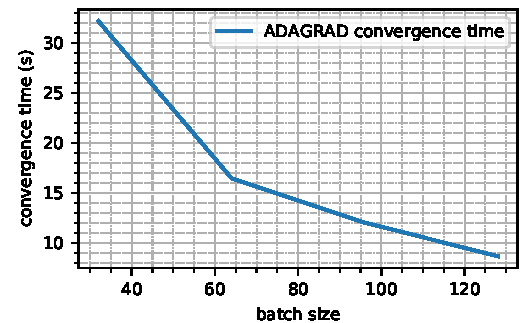
\includegraphics[scale=0.97,trim={0.0cm 0cm 0cm 0cm},clip]{./code/colabPlots/q3_adagrad_conv_time.pdf}\label{fig:q3_adagrad_conv_time}}\hspace{0.5cm}
	\subfloat[][ADAM: Convergence time, averaged over 10 runs, with increasing batch size]{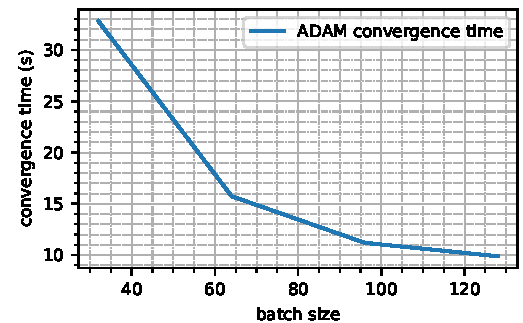
\includegraphics[scale=0.97,trim={0.0cm 0cm 0cm 0cm},clip]{./code/colabPlots/q3_adam_conv_time.pdf}\label{fig:q3_adam_conv_time}}
	\caption{Q3: CNN: Convergence time, averaged over 10 runs, with SGD, ADAGRAD and ADAM optimizer with increasing batch size}
	\label{fig:q3_conv_time}
\end{figure}
%%%%%%%%%%%%%%%%%%%%%%% CONVERGENCE TIME ALL %%%%%%%%%%%%%%%%%%%%%
\begin{figure}[!h]
	\centering
	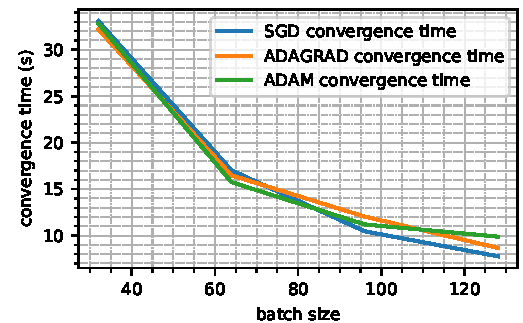
\includegraphics[scale=1.0,trim={0cm 0cm 0cm 0cm},clip]{./code/colabPlots/q3_all_conv_time.pdf}
	\caption{Q3: CNN: Convergence time comparison, averaged over 10 runs, with SGD, ADAGRAD and ADAM optimizer with increasing batch size}
	\label{fig:q3_all_conv_time}
\end{figure}


From Fig.~\ref{fig:q3_sgd_conv_time}, Fig.~\ref{fig:q3_adagrad_conv_time}, Fig.~\ref{fig:q3_adam_conv_time} and Fig.~\ref{fig:q3_all_conv_time}, we can see that as we increase the batch size the time taken to converge in seconds decreases which means learning becomes faster as we increase the batch size. However, this is opposite to the theoretical understanding we have on the effect of increasing batch size as we know if we increase the number of batch size, gradient computation time increases and thus learning time becomes slower. Thus, I believe, in this case, the CPU instructions or parallelization is playing a major role in deciding the convergence time. I have used \textit{time.time()} module of Python to compute the convergence time. I have also tested the code on Google Colab with GPU. Both CPU and GPU generated same trend of decreasing convergence time with increasing batch size. Therefore, I believe, here the convergence time (in seconds) is primarily governed by how the code execution is being handled by the CPU or GPU. I cross checked it with Professor and we agreed that it could be a possible reason of seeing this trend. Another possibility could be to plot iteration number instead of time in seconds on y-axis, however, we agreed to exclude that detail for this homework.
\newpage
\paragraph{Details gathered from a single run:} Fig.~\ref{fig:q3_loss_acc_32} shows the loss and accuracy for SGD, ADAGRAD and ADAM optimizers for a single run with batch size of $32$. The figures reveal that of all these three optimizers, ADAM performs best.
%%%%%%%%%%%%%%%%%%%%%%% CONVERGENCE TIME %%%%%%%%%%%%%%%%%%%%%
\begin{figure}[!h]
	\centering
	\subfloat[][Q3: CNN: Accuracy of different optimizer with 32 batch size]{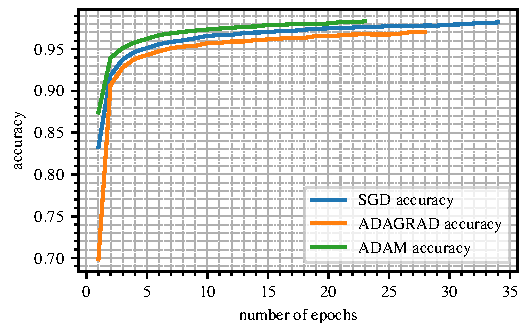
\includegraphics[scale=0.97,trim={0.0cm 0cm 0cm 0cm},clip]{./code/generatedPlots/q3_acc_batch_32.pdf}\label{fig:q3_acc_batch_32}}\hspace{0.5cm}
	\subfloat[][Q3: CNN: loss of different optimizer with 32 batch size]{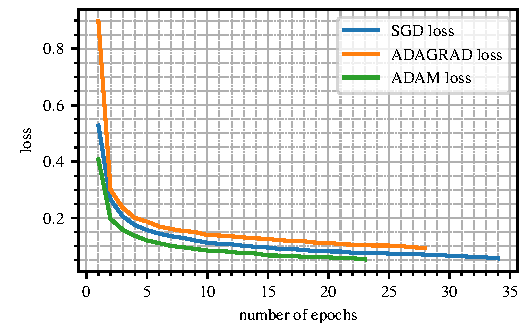
\includegraphics[scale=0.97,trim={0.0cm 0cm 0cm 0cm},clip]{./code/generatedPlots/q3_loss_batch_32.pdf}\label{fig:q3_loss_batch_32}}\hspace{0.5cm}
	\caption{Q3: CNN: Accuracy and loss with SGD, ADAGRAD and ADAM optimizer with increasing epoch with batch size of 32}
	\label{fig:q3_loss_acc_32}
\end{figure}
Fig.~\ref{fig:q3_loss_acc_64} shows the loss and accuracy for SGD, ADAGRAD and ADAM optimizers for a single run with batch size of $64$. The figures reveal that of all these three optimizers, ADAM performs best.
%%%%%%%%%%%%%%%%%%%%%%% CONVERGENCE TIME %%%%%%%%%%%%%%%%%%%%%
\begin{figure}[!h]
	\centering
	\subfloat[][Q3: CNN: Accuracy of different optimizer with 64 batch size]{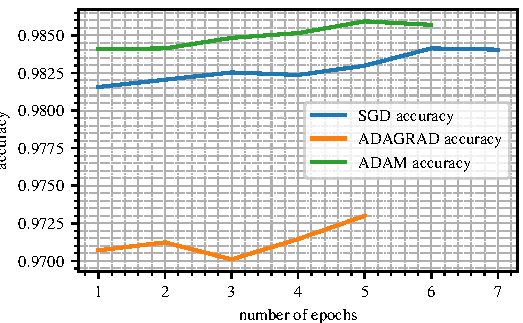
\includegraphics[scale=0.97,trim={0.0cm 0cm 0cm 0cm},clip]{./code/generatedPlots/q3_acc_batch_64.pdf}\label{fig:q3_acc_batch_64}}\hspace{0.5cm}
	\subfloat[][Q3: CNN: loss of different optimizer with 64 batch size]{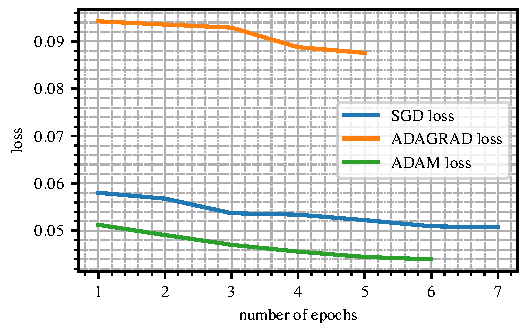
\includegraphics[scale=0.97,trim={0.0cm 0cm 0cm 0cm},clip]{./code/generatedPlots/q3_loss_batch_64.pdf}\label{fig:q3_loss_batch_64}}\hspace{0.5cm}
	\caption{Q3: CNN: Accuracy and loss with SGD, ADAGRAD and ADAM optimizer with increasing epoch with batch size of 64}
	\label{fig:q3_loss_acc_64}
\end{figure}
Fig.~\ref{fig:q3_loss_acc_96} shows the loss and accuracy for SGD, ADAGRAD and ADAM optimizers for a single run with batch size of $96$. The figures reveal that of all these three optimizers, ADAM performs best.
%%%%%%%%%%%%%%%%%%%%%%% CONVERGENCE TIME %%%%%%%%%%%%%%%%%%%%%
\begin{figure}[!h]
	\centering
	\subfloat[][Q3: CNN: Accuracy of different optimizer with 96 batch size]{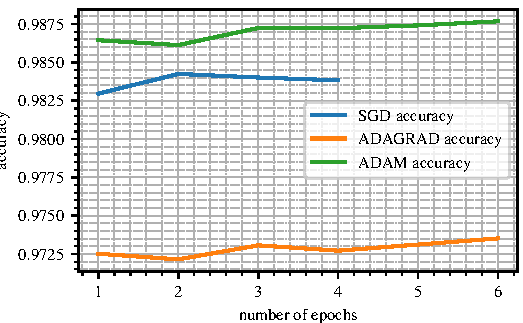
\includegraphics[scale=0.97,trim={0.0cm 0cm 0cm 0cm},clip]{./code/generatedPlots/q3_acc_batch_96.pdf}\label{fig:q3_acc_batch_96}}\hspace{0.5cm}
	\subfloat[][Q3: CNN: loss of different optimizer with 96 batch size]{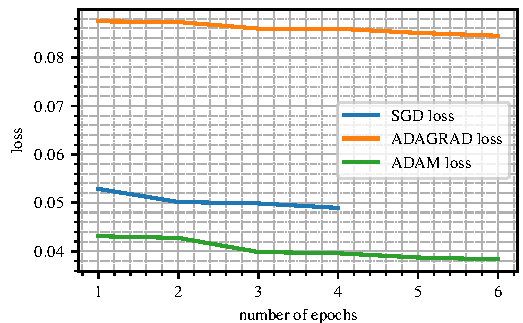
\includegraphics[scale=0.97,trim={0.0cm 0cm 0cm 0cm},clip]{./code/generatedPlots/q3_loss_batch_96.pdf}\label{fig:q3_loss_batch_96}}\hspace{0.5cm}
	\caption{Q3: CNN: Accuracy and loss with SGD, ADAGRAD and ADAM optimizer with increasing epoch with batch size of 96}
	\label{fig:q3_loss_acc_96}
\end{figure}
Fig.~\ref{fig:q3_loss_acc_128} shows the loss and accuracy for SGD, ADAGRAD and ADAM optimizers for a single run with batch size of $128$. The figures reveal that of all these three optimizers, ADAM performs best.
%%%%%%%%%%%%%%%%%%%%%%% CONVERGENCE TIME %%%%%%%%%%%%%%%%%%%%%
\begin{figure}[!h]
	\centering
	\subfloat[][Q3: CNN: Accuracy of different optimizer with 128 batch size]{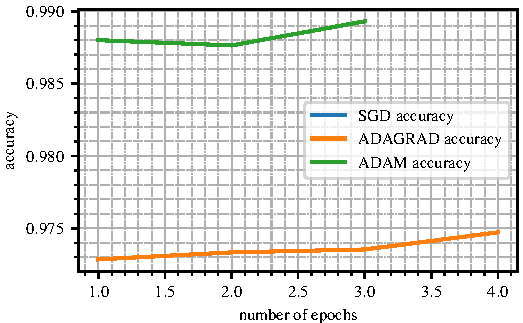
\includegraphics[scale=0.97,trim={0.0cm 0cm 0cm 0cm},clip]{./code/generatedPlots/q3_acc_batch_128.pdf}\label{fig:q3_acc_batch_128}}\hspace{0.5cm}
	\subfloat[][Q3: CNN: loss of different optimizer with 128 batch size]{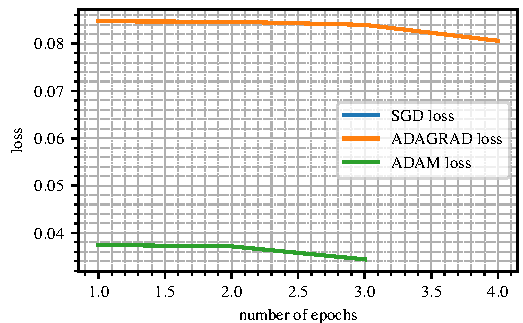
\includegraphics[scale=0.97,trim={0.0cm 0cm 0cm 0cm},clip]{./code/generatedPlots/q3_loss_batch_128.pdf}\label{fig:q3_loss_batch_128}}\hspace{0.5cm}
	\caption{Q3: CNN: Accuracy and loss with SGD, ADAGRAD and ADAM optimizer with increasing epoch with batch size of 128}
	\label{fig:q3_loss_acc_128}
\end{figure}